\lab{Algorithms}{Conformal Maps}{Conformal Maps}

\objective{To become familiar with some of the basic properties of conformal maps and some of their basic applications.}

The analysis of complex valued functions has been called ``one of the most beautiful and useful fields of mathematics.''  Conformal maps are special functions in complex analysis that have proven to be very useful in several applications, especially those that model physical phenomena.

\section*{Polar Representation of Complex Numbers}

One of the most important results in Complex Analysis is Euler's Formula. It states that: 

$$e^{i\theta}=cos(\theta)+i sin(\theta)$$.

One way to derive this important result is to consider the taylor series expansion of each of the functions involved. 

From this formula, we can see that $e^x$ maps the imaginary axis onto the unit circle on the complex plane. From our knowledge of the sine and cosine functios, we can also know that this mapping has a period of $2\pi$. From here, notice that we may represent any number on the complex plane in the form $r e^{i\theta}$ for $r\geq 0$ and $0 \leq \theta \leq 2\pi$. This is what is known as the polar representation of a complex number. It is identical to the polar representation of points in the standard cartesian plane, except for the use of the function $e^x$. The number $\theta$ is known as the argument, or phase, of a complex number. The number $r$ is known as the modulus, magnitude, or absolute value of a complex number. In the complex plane we define $|z|$ as the modulus of $z$ and $arg(z)$ as the argument of $z$. These functions are implimented in python through the abs() and sp.arg() functions. 

In python we can make a complex number using the complex() function. For example a=complex(1,2) assigns the value of a to $1+2i$.

In scipy the functions sp.real() and sp.imag() return the real and immaginary parts of a complex number respectively. 


\begin{problem}
Write a function which accepts a complex number $z$ and returns the ordered pair $(r,\theta)$ corresponding to the polar representation of $z$. Include a special case for $z=0$. Use the built in real part and imaginary part functions, not the modulus and argument functions. 
\end{problem}

\section*{Conformal Maps}

We begin by examining some maps on the complex plane.  Let
\[
f(z) = \frac{3z - 4}{z - 2}
\]
and
\[
g(z) = z^2 - 2
\]
What happens if we map the box $[0,1]\times[0,i]$ under these mappings?  
\newpage
Looking at $g(z)$, we see the box turn into a sort of curved triangle.  On the other hand, if we look at $f(z)$, it seems like there is even more distortion than in the case of $g(z)$.
\begin{figure}
\begin{center}
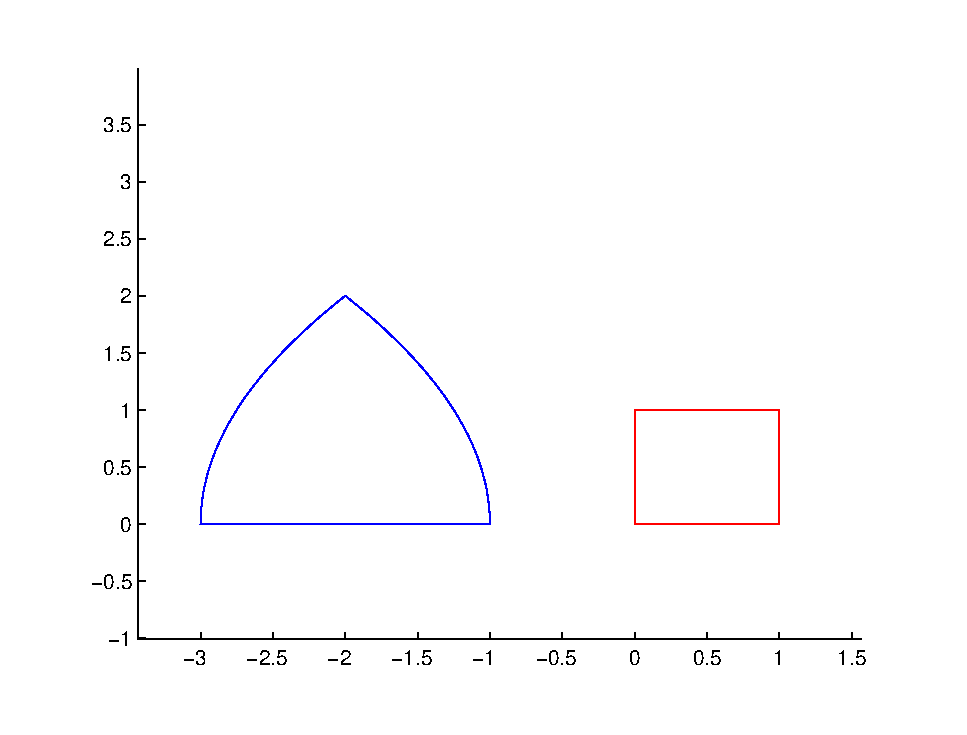
\includegraphics[scale=0.5]{map1}
\caption{The box $[0,1]\times[0,i]$ under g(z).  The vertical axis is the imaginary line and the horizontal axis is the real line.}
\end{center}
\end{figure}

\begin{figure}
\begin{center}
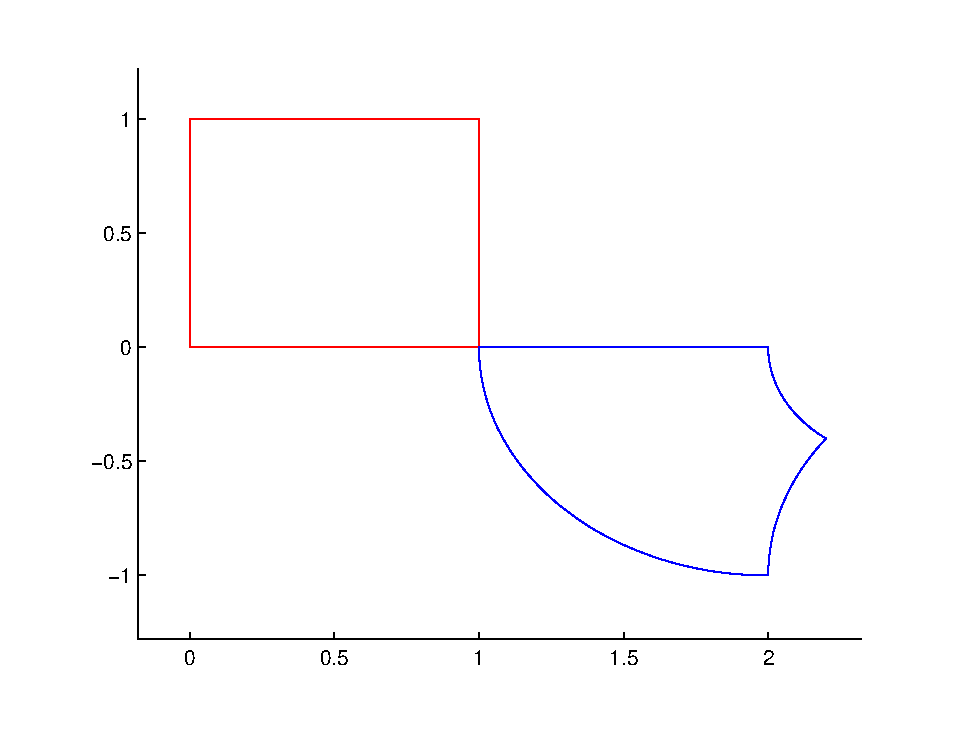
\includegraphics[scale=0.5]{map2}
\caption{bla bla bla}
\end{center}
\end{figure}

There is a fundamental difference between these two mappings.  Though in both cases the shape is significantly distorted, in the case of $f(z)$ the angles where two sides meet are preserved, whereas $g(z)$ distorts not only the shape of the lines but also the angles where they meet.  Maps that preserve angles, as in the case of $f(z)$, are called conformal.

\begin{figure}
\begin{center}
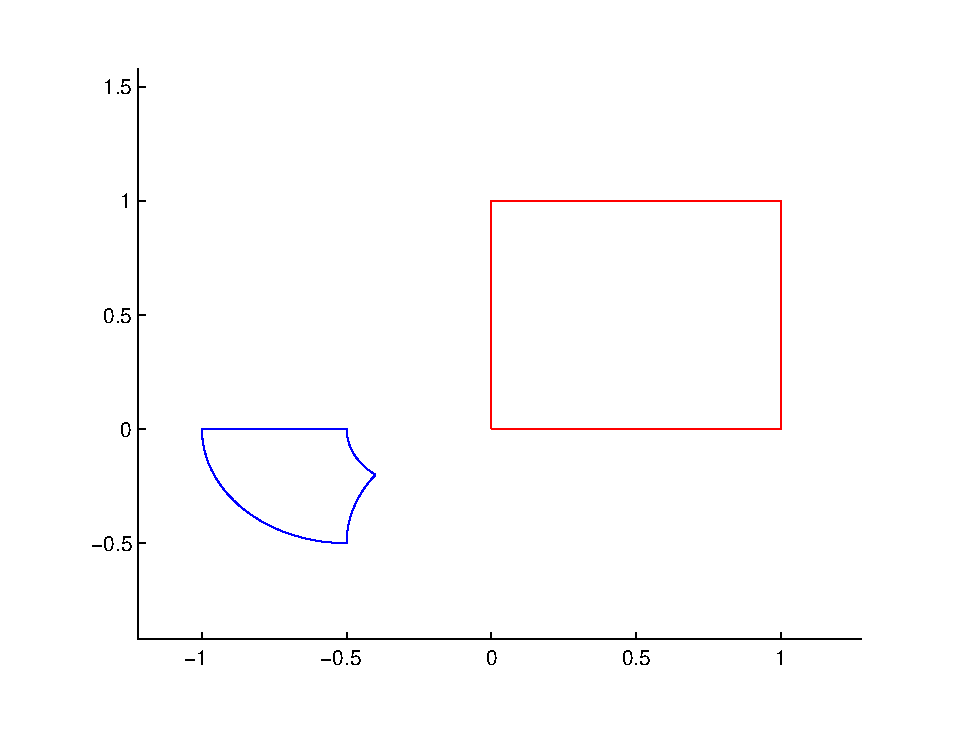
\includegraphics[scale=0.33]{map3}
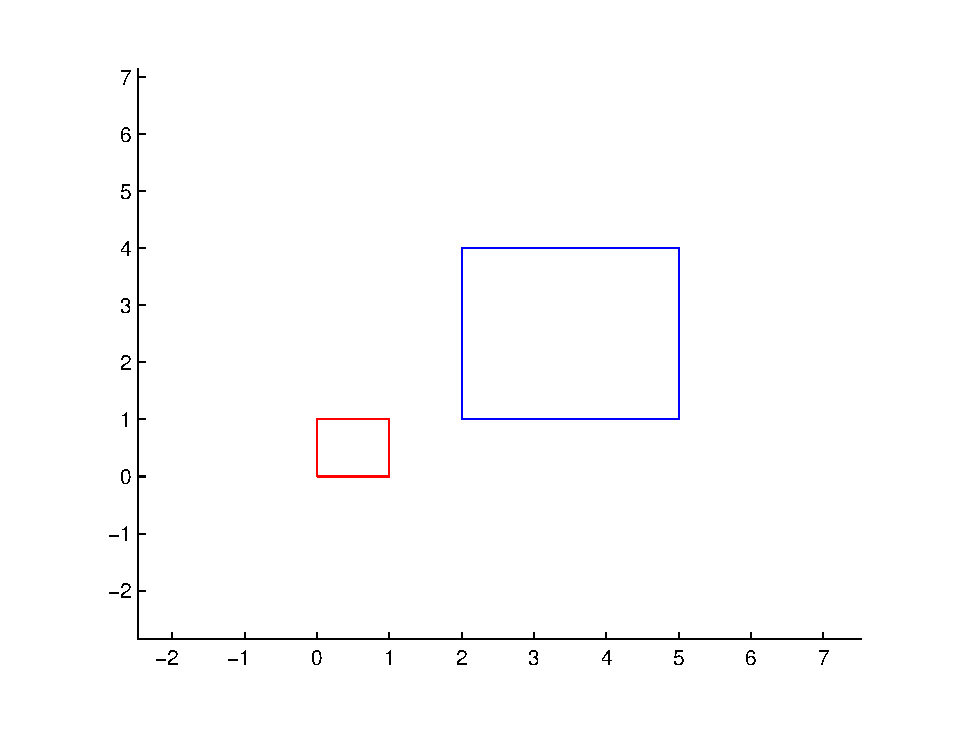
\includegraphics[scale=0.33]{map4}
%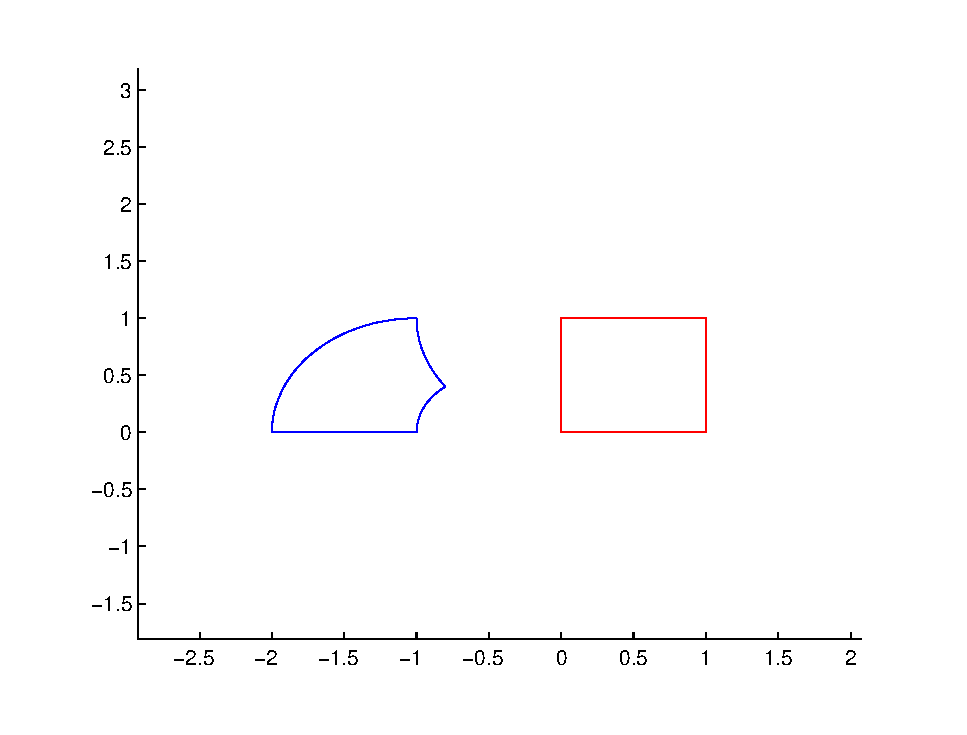
\includegraphics[scale=0.33]{./Applications_Labs/ConfMaps/map5}
\caption{Some more conformal maps}
\end{center}
\end{figure}

\begin{problem}
Write a Python script that transform a shape on the complex plane using the the conformal maps that we have used in the examples.  What do you expect will happen to the unit circle on the complex plane under these transformations?  Do your predictions match the results?  Try this for several shapes.
\end{problem}

\section*{Holomorphic and Analytic Functions}

We will now briefly introduce the idea of holomorphic and analytic functions. Again, there is a lot of heighly developed theory behind these types of functions.

A complex valued function is said to be holomorphic at a point in the complex plane if it is complex differentiable at all points within some arbitrarily small distance of that point. This means that the limit $lim_{\Delta z \to 0} \frac{f(z+\Delta z)-f(z)}{\Delta z}$ exists and is finite. We say that a complex function is holomorphic at some point of the complex plane if it is complex differentiable for all points that are within some nonzero distance of that point. We say a function is holomorphic on a set if it is holomorphic at every point in the set.

A term that is more commonly used to refer to these functions is "Analytic." Generally a function is said to be analytic at a point if it is equal to a convergent power series within some arbitrarily small distance of that point. It can be proven that all holomorphic functions are analytic and that that all functions that are complex analytic are also holomorphic.

A useful result concerning holomorphic functions and conformal mappings is that a holomorphic function with a nonzero derivative on a given complex domain is also conformal on that domain. Strictly speaking, a set is said to be a domain in the complex plane if it contains none of its boundary points and if it lies in one connected whole. There is a more proper definition of connectivity as well, but we will not introduce it here.

Why all the trouble about holomorphic functions? Being holomorphic turns out to be a reasonably strict constraint on a complex function which allows us to know many things about its behavior, for example, any function that is holomorphic on a domain is also infinitely differentiable on that domain. It is a very useful property in both theoretical and real-world applications. There are specific applications in electrostatics, fluid flow, and many other fields.

One of the quickest ways to tell if a function is complex differentiable is that the real and imaginary parts of the function satisfy the Cauchy-Riemann Equations. To explore the meaning of this phrase, consider the function $f(z)$ on some domain of the complex plane. Let $z=x+i y$ where $x=Re(z)$ and $y=Im(z)$. We may rewrite $f(z)$ in the following form: $$f(z)=f(x+i y)=u(x,y)+i v(x,y)$$ where $u$ and $v$ are two unique real valued functions of two real variables. $f(z)$ will be complex differentiable at a point if and only if the two functions $u$ and $v$ are differentiable at that point and satisfy the equations $$\frac{\partial u}{\partial x}=\frac{\partial v}{\partial y}$$ and $$\frac{\partial u}{\partial y}=-\frac{\partial v}{\partial x}$$

\begin{problem}
Write a function which tests the following complex functions to determine whether or not they are complex diferentiable at a given point z. Do this by taking a sampling of points in a very small circle around z and using each of them to estimate the limit $lim_{\Delta z \to 0} \frac{f(z+\Delta z)-f(z)}{\Delta z}$. Then depending on whether or not the points all give a similar estimate for the limit, have the function return either "differentiable" or "not differentiable." 

Use your function to test the following functions for differentiability

$Re(z)$ at $z=1+ i$

$z Re(z)$ at $z=0$ and at $z=1+ i$

$e^z$ at $\pi i$

$sin(x) cosh(y) + i cos(x) sinh(y)$ at $\pi i$

$sin(x) cosh(y) - i cos(x) sinh(y)$ at $\pi i$
\end{problem}

It follows from the Cauchy-Riemann Equations that if $f$ is holomorphic on a domain, the functions $u$ and $v$ are conjugate harmonic functions on that domain. This means that both $u$ and $v$ satisfy the Cauchy-Riemann Equations and Laplace's equation, which says that: $$\frac{\partial^2 u}{\partial x^2}+\frac{\partial^2 u}{\partial y^2}=0$$ and that: $$\frac{\partial^2 v}{\partial x^2}+\frac{\partial^2 v}{\partial y^2}=0$$. 

\begin{problem}
Prove that for $u$ and $v$ as defiined above, if $f$ is analytic on a domain, then $u$ and $v$ will be conjugate harmonic on that domain.
\end{problem}

The theory of holomorphic functions and conformal mappings is highly developed and well studied.  Here we only scratch the surface and comment on an important theorem for applications that will be useful in later volumes.

\section*{The Schwarz-Christoffel Transformation}
This transformation is very useful in applications of complex analysis.  Once again, the theory behind this is very rich, and we only state a theorem and look at some simple implications here.

\begin{theorem}  Let $P$ be a polygon on the complex plane having consecutive corners at $z_1, z_2, ..., z_n$ with corresponding right turn angles $\theta_1, \theta_2,...\theta_n$.  Then there exists a function that is a one to one conformal map from the upper half plane onto the interior of $P$ of the form:
\[
f(z) = A\int_0^z (\zeta - x_1)^{\frac{\theta_1}{\pi}}..(\zeta - x_{n-1})^{\frac{\theta_{n-1}}{\pi}}d\zeta + B
\]
Where $\theta_i$ represents the angle made by adjacent sides of the polygon and $x_i \in \mathbb{R}$.
\end{theorem}

We omit the proof here.  Consider the power of this theorem - we are able to map the upper half of the complex plane onto a polygon of our choosing.  This is very powerful for finding the numerical solutions to differential equations that model physical systems.  It turns out that a conformal mapping retains sufficient structure of a domain so that a solution in a transformed domain will be the same as the solution in the original domain.  This fact along with the theorem allows us to take problems which may be very difficult to solve in one domain and transform the domain to a polygonal domain of our choosing where a solution is much easier to find.  We give an example of such a transformation using built in Python functions:

\begin{example}
We will give an example showing how to find a Schwarz-Christoffel transform.  Suppose we wish to transform the upper half plane onto the triangle with corners at $0, i,$ and $1$.  We choose $x_1 = -1$ and $x_2 = 1$.  Starting from the upper corner, we have $\theta_1 = \theta_2 = \frac{-3\pi}{4}$ and $\theta_3 = \frac{-\pi}{2}$.  Using theorem 36.1, we have an expression for our mapping:
\begin{align*}
f(z) &= A\int_0^z(\zeta + 1)^{\frac{-3}{4}}(\zeta - 1)^{\frac{-3}{4}}d\zeta + B \\
	 &= A\int_0^z(\zeta^2 - 1)^{\frac{-3}{4}}d\zeta + B
\end{align*}

\end{example}

\begin{problem}
Find the conformal map that transforms the upper half plane to the strip $|Re(z) < 1|, Im(z) > 0$.  Display the result in a meaningful way.
\end{problem}
